\question 输入受限的双端队列是指元素只能从队列的一端输入,但可以从队列的两端输出,如图所示。若有8、1、4、2依次进入输入受限的双端队列,则得不到输出序列(
~)。~

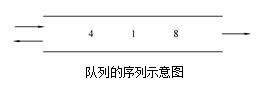
\includegraphics[width=2.75000in,height=0.97917in]{computerassets/95a34a22ed1cd42d10a23b488d7f98e8.png}
\par\fourch{2、8、1、4}{1、4、8、2}{4、2、1、8}{\textcolor{red}{2、1、4、8}}
\begin{solution}A选项:首先,8、1、4、2都从左端入队,然后2从左端出队,8从右端出队,1从右端出队,4从左端出队,得到A的序列。
B选项:首先,8和1分别从左端输入,然后1从左端出队,4再从左端入队,4再从左端出队,2从左端入对,8从右端出队,2从左端出队,得到B的序列。
C选项:首先,8、1、4都从左端入队,4从左端出队,2再从左端入队,2从左端出队,1从左端出队,8从左端或者右端出队,得到C的序列。
D选项:首先,8、1、4、2都从左端入队,然后2从左端出队,队列的序列变成如图所示,接着如果要让1出队列,必须4或8先出队列,所以D的序列不可能实现。

~
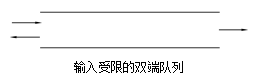
\includegraphics[width=2.67708in,height=0.85417in]{computerassets/5165378b619f5b040e98b8bafb986fda.png}
\end{solution}
